\hypertarget{section-building-block-view}{%
\section{5 Building Block View}\label{section-building-block-view}}

This section shows the static decomposition of the system into building blocks (e.g. modules, components, subsystems, classes, interfaces, packages, libraries, frameworks, layers, partitions, tiers, functions, operations, \ldots) including their relationships and associations. It helps to maintain an overview of your source code by making its structure understandable through abstraction.

\subsection{Frontend}
\subsubsection{Component-Based Frontend Architecture}
The Vivendo webshop frontend follows a \textbf{component-based modular frontend design}. The different modules are interconnected to provide a seamless shopping experience. The primary technologies used include \textbf{Next.js, Tailwind CSS}, API integration and Context API for state management. This approach ensures:
\begin{itemize}
    \item Clear separation of concerns through distinct modules.
    \item Reusability of components across different sections.
    \item Better maintainability and scalability.
    \item Efficient state and API management.
\end{itemize}
The architectural overview is depicted in the figure below:

\begin{figure}[h]
    \centering
    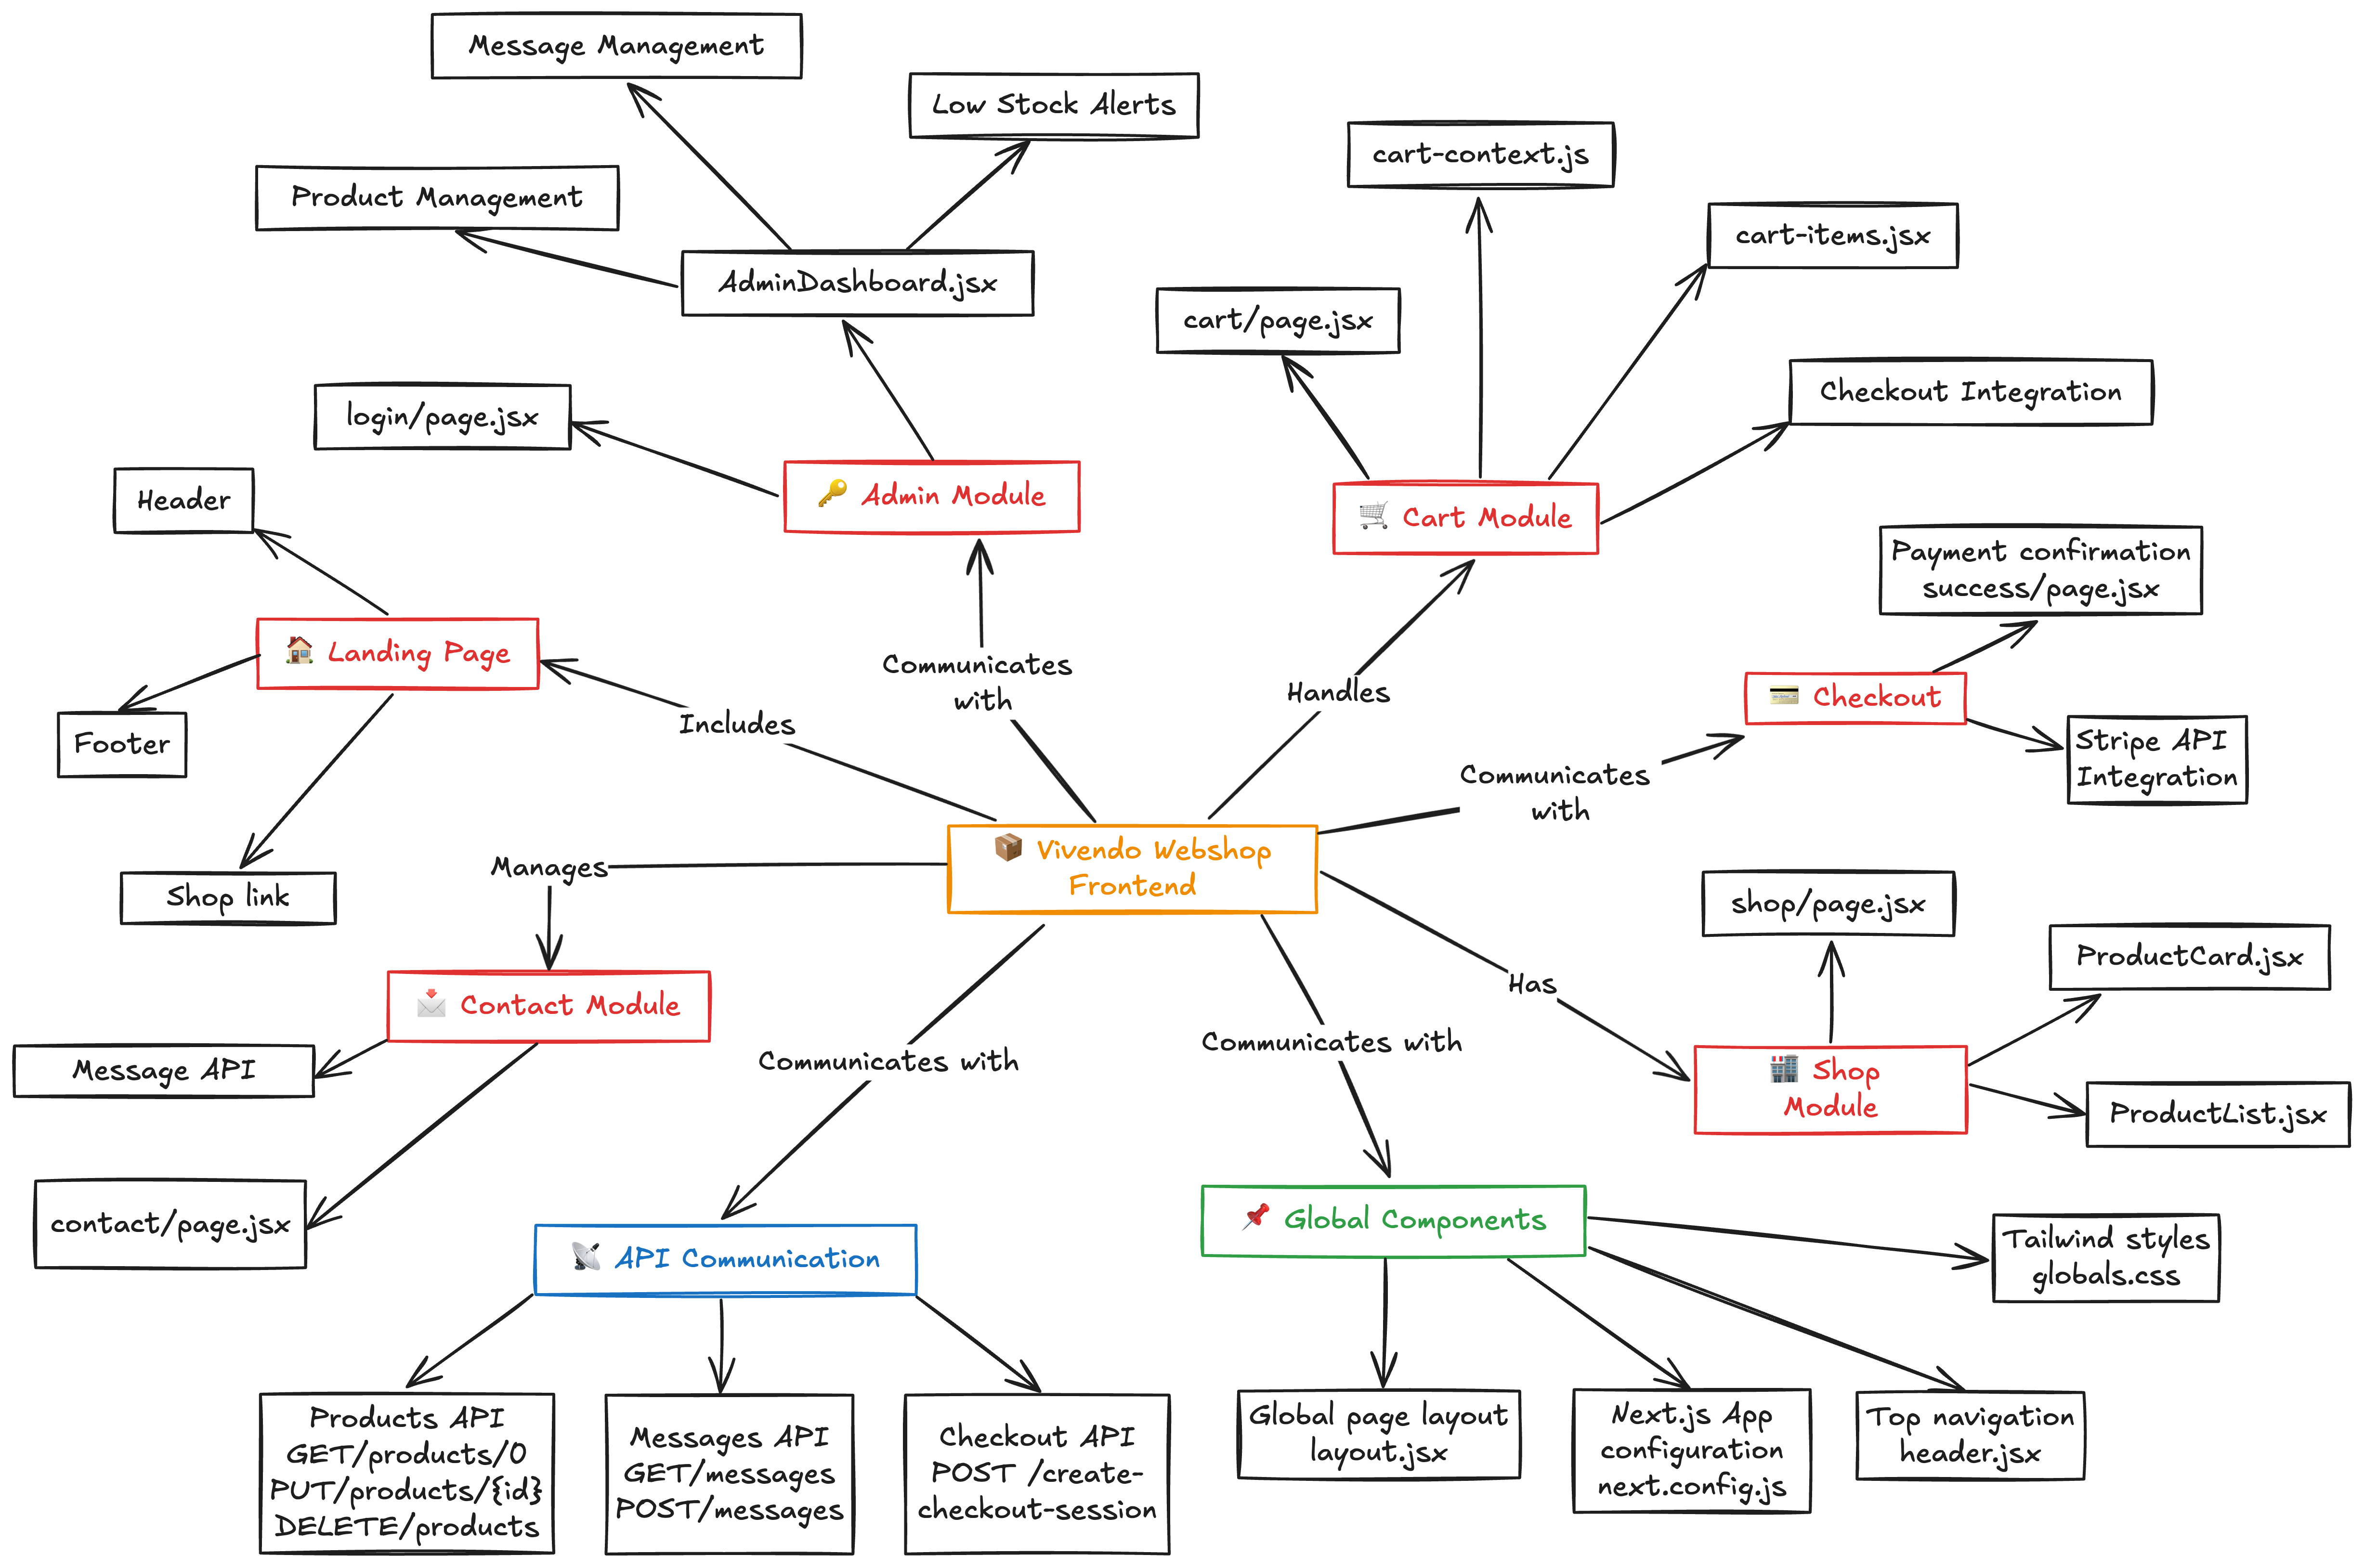
\includegraphics[width=\textwidth]{images/New_frontend_architecture.png}
    \caption{Component-Based Frontend Architecture}
    \label{fig:architecture}
\end{figure}

\subsubsection{Core Frontend Modules and Interactions}
The system consists of several modules:
\begin{itemize}
    \item \textbf{Landing Page Module}: Includes key UI components such as the header, footer and navigation links.
    \item \textbf{Admin Module}: Manages the admin dashboard, including product management, low stock alerts and message management. The admin module is responsible for managing products, messages, and stock alerts. It is connected to the \textbf{Admin Dashboard} component, which communicates with the API layer.
    \item \textbf{Cart Module}: Handles cart functionality, including cart context, cart items and checkout integration. The cart module manages cart-related functionalities and state using \texttt{cart-context.js}. It also connects with the checkout module to handle Stripe payments.
    \item \textbf{Shop Module}: Displays product listings and product cards with interactivity.
    \item \textbf{Checkout Module}: Integrates with Stripe API for handling payments and success confirmations.
    \item \textbf{Contact Module}: Manages user interactions via the contact page and handles message submissions. It connects with the API layer to store and retrieve messages.
    \item \textbf{API Communication Layer}: Manages requests to the backend services, including product APIs, messages API and checkout API. This layer serves as the middleware between the frontend and backend, making requests via REST APIs. It handles product data, message submissions, and checkout sessions.
    \item \textbf{Global Components}: Includes shared layout elements, styles and configurations.
\end{itemize}


%% ADD BACKEND BUILDING BLOCK VIEW PART / ARCHITECTURE HERE

\subsection{Backend}
